\documentclass[12pt]{article}
\usepackage{hyperref} 
\usepackage{titling}
\usepackage{xcolor}
\usepackage[a4paper,margin=1in]{geometry}
\usepackage{fancyhdr}
\usepackage{graphicx}
\usepackage{tabto}
\pagestyle{fancy}
\setcounter{tocdepth}{4}
\setcounter{secnumdepth}{4}
\chead{Final Report}
\lhead{}
\rhead{}
\graphicspath{ {./images/} }
\definecolor{light-gray}{gray}{0.95}
\newcommand{\code}[1]{\colorbox{light-gray}{\texttt{#1}}}
\usepackage{pdfpages}

\begin{document}
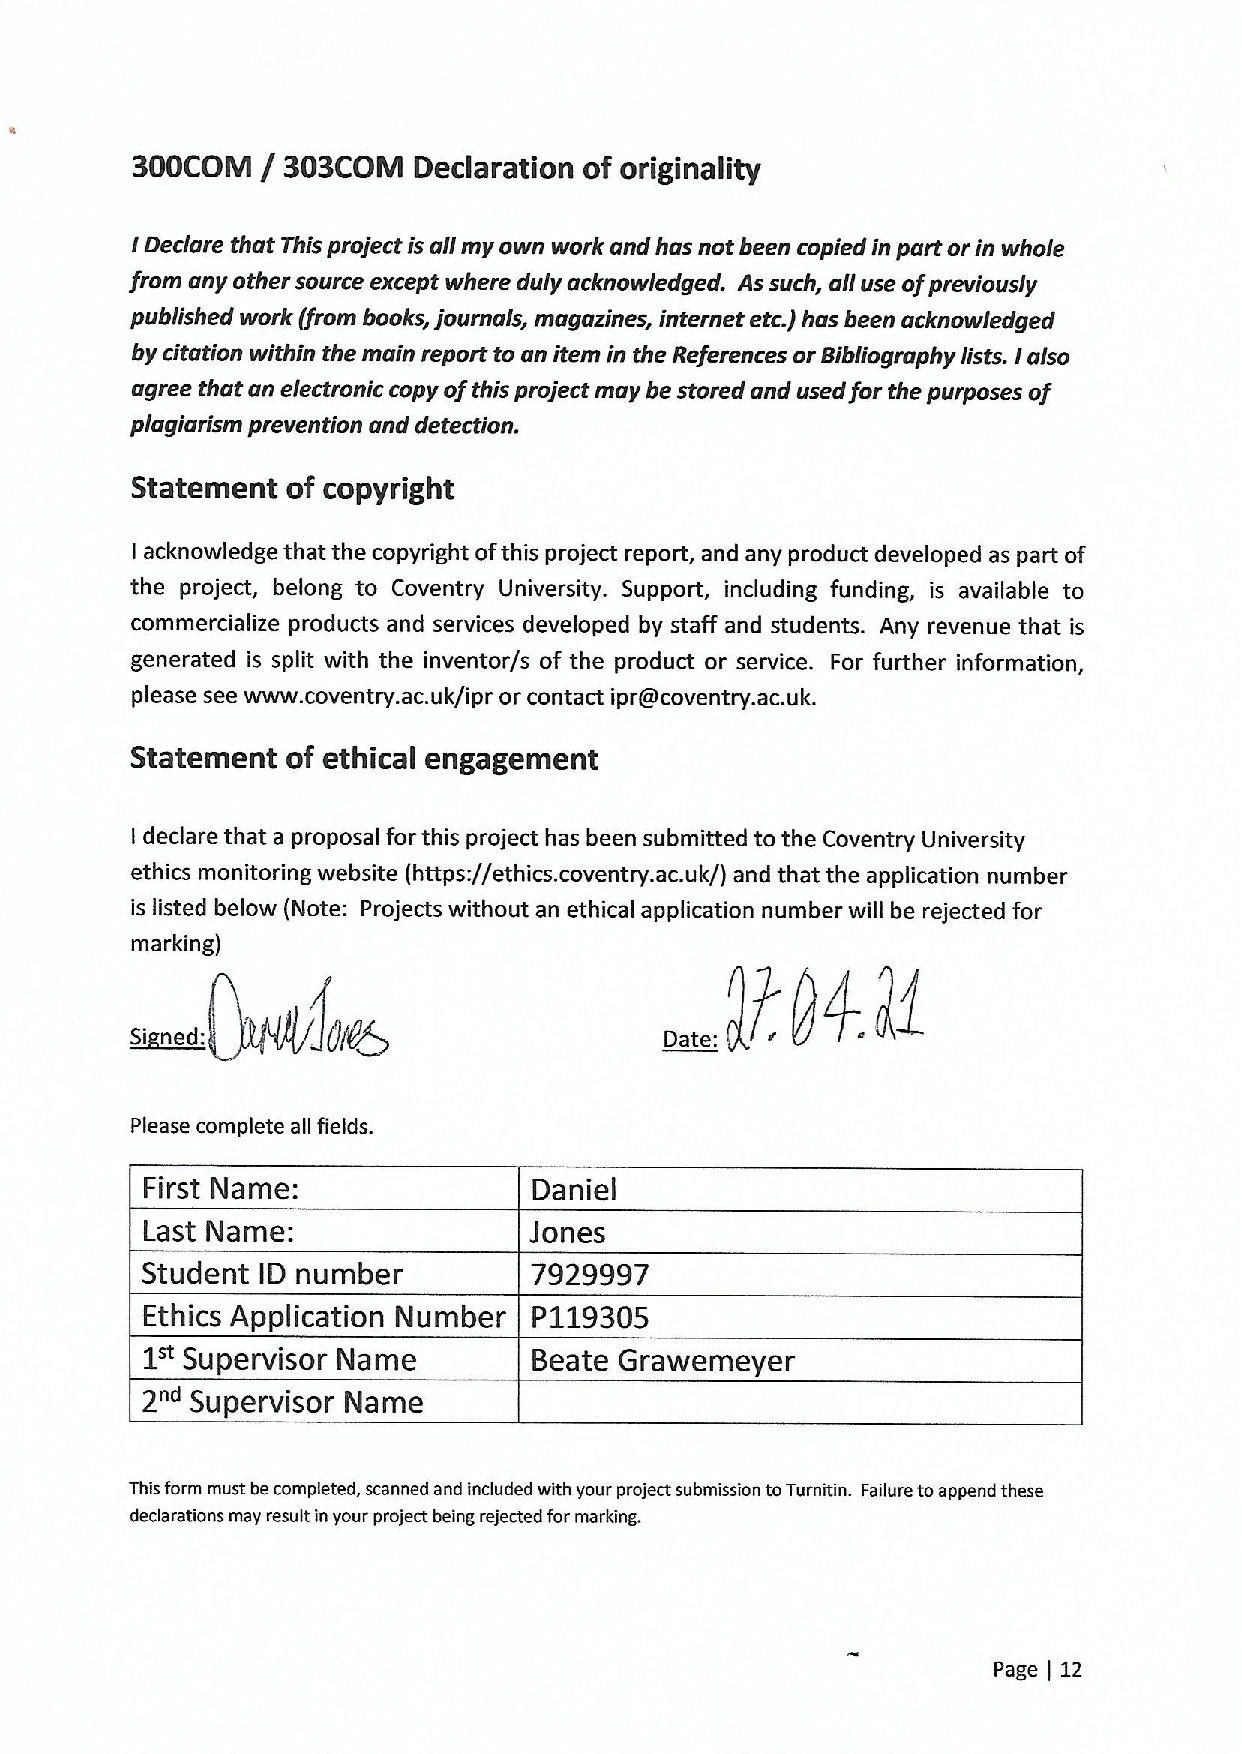
\includepdf[pages=-]{SER_Daniel_Jones_Declaration.pdf}
\begin{center}
	\vspace*{1cm}
	\Huge \textbf{A Speech Emotion Recognition Classifier to Aid Performance Review in Learning Environments} \\[1em]
	\vspace{5cm}
	\LARGE \textbf{Daniel G. Jones}
	\\
	\vspace{0.3cm}
	\large jonesd37@coventry.ac.uk
	\\
	\large Student ID: 7929997
	\\
	\vspace{3cm}
	\large Supervised by \textbf{Dr. Beate Grawemeyer}
	\\
	\vspace{0.3cm}
	\large ac7655@coventry.ac.uk
	\\
	\vspace{3cm}
	\large Submitted to the School of Computing, Engineering and Mathematics Coventry University
\end{center}
\newpage
\tableofcontents
\newpage
\section{Abstract}

Classifying human emotion from speech is a challenging problem that has the potential to benefit various fields in different ways. One such field is in learning environments, where the application of such technology could aid in matters such as performance review / analysis or in helping children with special needs, such as autism. In this project, a speech emotion classification model has been built and trained on the Ryerson Audio-Visual Database of Emotional Speech and Song (RAVDESS), and then deployed in the form of a graphical tool that analyses either pre-recorded audio or a live audio input and outputs the weighted predictions. The model has been developed using a 2-Dimensional Convolutional Neural Network (CNN) approach, where the training data is in the form of audio files converted into Mel Spectrograms. Through this approach, an exact prediction accuracy of 68.8\% (and binary positive / negative accuracy of 94\%) has been achieved on an unseen test dataset, with further personalised tests yielding promising results.

\section{Acknowledgements}

With thanks to my project supervisor, Dr. Beate Grawemeyer, for the initial inspiration and constant support throughout the project.
\\

\noindent With thanks to my friend Céline Capelli of ETH Zürich for testing the application, providing useful audio data for testing, and for providing her unique perspective.
\\

\noindent With thanks to my partner Hannah Vogt of the Pädagogische Hochschule Zürich for her love, inspiration, motivation, and for imparting the insights of a primary school teacher. 
\\
\newpage

\section{Introduction}

It can be observed that technology has yet to make a significant contribution towards aiding performance review in learning environments and indeed learning environments on the whole. This can largely be attributed to the lack of effectiveness of the existing tools, whereby much of the information obtained is neither insightful nor particularly meaningful.
\\

\noindent Traditional approaches to the incorporation of technology in learning environments have tended to focus more on interactivity as opposed to analysis, which has resulted in a lack of progress in the areas of performance review, analysis, and overall utility (Cho et al. 2020). This is due in part to the complexity of such environments, with many subjective metrics and mediums that, at first glance, appear to be difficult to study and quantify.
\\

\noindent In this project, speech emotion has been identified and selected as a suitable metric for analysis. Speech emotion is a language agnostic metric that transcends many of the barriers posed by the more obvious metrics such as spoken / body language or facial expressions.
\\

\noindent Despite the many nuances of speech, such as tonality or pitch, there are clear patterns that can be derived from studying how emotions are conveyed. A spectrogram is a visual representation of the spectrum of frequencies (in this case, the frequencies are converted to the mel scale) across a signal as a function of time. Consider the following mel spectrograms produced from two different male actors saying a short sentence in a blatantly angry and then sad manner.
\\
\\
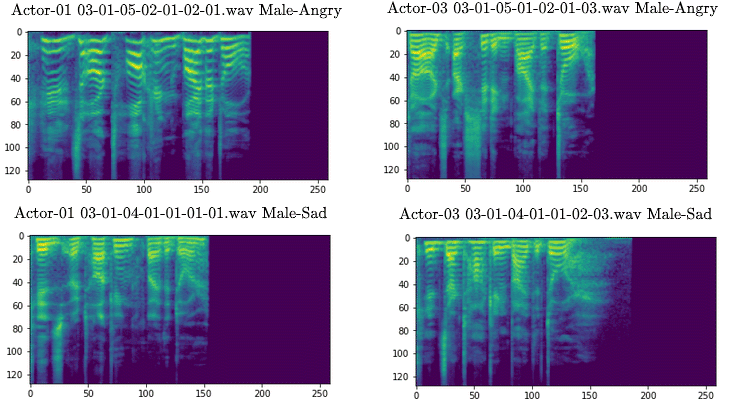
\includegraphics[width=14cm]{figure_1_spectrogram_comparison}

\noindent Figure 1: Spectrogram comparison
\vspace{0.05cm}

\noindent Even from a macro perspective, it is possible to make out some visible similarities. Take for example the large circular shapes that can be made out from the two angry clips, or the distribution of the yellow (corresponding to pitch across the mel scale) lines in the sad clips. The spectrogram is represented by a matrix of values, which is where the vast, more subtle patterns can be identified and observed - making it an ideal candidate for a CNN approach.

\newpage

\noindent Prior to the increased popularity of machine learning, conventional methods for analysing and processing speech involved the usage of Gaussian Mixture Models (GMM) and Hidden Markov Models (HMM), both of which produced results that were simply too inaccurate to ever put into production (Sainath et al., 2013; Venkataramanan \& Rajamohan, 2019). The accessibility of machine learning techniques has lead to novel approaches such as the application of Recurrent Neural Networks (RNN) and CNNs, resulting in improved accuracy and introducing completely different approaches to the problem.
\\

\noindent In this paper, inspired by the notable success and improvements seen from the application of CNNs in particular, a relatively accurate classification model has been trained through applying CNNs to Mel Spectrogram representations of audio files. The Mel Spectrogram effectively allows us to transform the classification problem from the audio domain into the visual domain, where CNNs excel. As previously shown in figure 1, there are many subtle patterns to be found in the data, but it is a difficult task to manually calculate and label these ourselves. Hence a deep learning approach, where the model learns to recognise and extract features itself, becomes a clear suitable choice.
\\

\noindent The final trained model has then been deployed into a general purpose graphical tool that can perform predictions across pre-recorded audio files or through recording on the fly. The graphical tool has been purposefully designed with simplicity in mind, with the intention of being easy to use and incorporate into learning environments.

\section{Literature Review}

\subsection{\href{https://www.intechopen.com/books/social-media-and-machine-learning/automatic-speech-emotion-recognition-using-machine-learning}{Automatic Speech Emotion Recognition Using Machine Learning}}
Automatic Speech Emotion Recognition Using Machine Learning takes a comparative look at SER systems. The underlying method to extract and process the speech signals (using Mel-frequency cepstrum coefficients and modulation spectral features in conjunction with feature selection) remains the same whilst the machine learning paradigms differ. The paper first looks at a recurrent neural network approach and goes on to compare it against both multivariate linear regression and support vector machine approaches. The paper makes the claim that such approaches were selected due to their existing popularity in the field. 
\\

\noindent The initial criticism of the paper is that it fails to consider the convolutional neural network (CNN) approach, despite its notable popularity and differences to the other methods. However, the paper is still concise and informative enough to warrant a full review. One positive quality that immediately stands out is how clear the information is presented, both in terms of looks and in use of language. An additional outstanding quality of this paper is the lack of pre-requisite knowledge required of the reader; many similar such papers assume at least a fundamental understanding and generally a lot more, whilst this paper describes most of the necessary knowledge required to grasp the content.
\\

\noindent The paper starts by explaining the importance behind SER technology, the main argument can be reduced to how effective and convenient it is to obtain information pertaining to the emotional state of an individual in comparison to other methods (such as facial expressions and physiological signals). This argument can be applied to the idea of using such technology in learning environments based on the documented effectiveness of the results in similar scenarios. The paper even uses learning environments as an example of a potential application of such technology; Kerkeni et al. (2019) state that ``a teacher can use SER to decide what subjects can be taught and must be able to develop strategies for managing emotions within the learning environment''.
\\

\noindent The authors then describe their system from a top-down perspective, this includes which emotions are in scope as well as the decision making process behind which algorithms are selected. It appears that the researchers were restricted by their datasets as to which emotions ended up in-scope. Whilst this does not affect the content of this particular paper, a more careful consideration will have to be made when applying this to learning environments (as per this project).
\\

\noindent Delving further into the paper, the authors describe how the different algorithms are applied to solve the problem, which is achieved by mathematical notation and descriptions of important variables. This is of course a necessity for such a paper, although the notation is clear enough for even those with weaker mathematical backgrounds to gain insight. The paper concludes by displaying and contrasting between the results obtained from the experiments; the main conclusion is that SER produces the best recognition results with a limited dataset whilst RNN performs better when a higher volume of data is available. Such results will prove vital when comparing against and assessing the effectiveness of our SER system.

\subsection{\href{https://www.mdpi.com/1424-8220/20/1/183/pdf}{A CNN-Assisted Enhanced Audio Signal Processing for Speech Emotion Recognition}}
Due to the notable omission of a CNN approach in the first reviewed paper, this paper has primarily been selected to gain practical insight into such an approach. The paper starts by defining the motivation behind it, using similar arguments to the previously reviewed paper. One particular area of interest is the point about ``extracting hidden information'', where Kwon (2020) refers to uncovering previously undetected, new information using a CNN approach. At first glance, it appears that the author looks at the issue more through the lens of human computer interaction (HCI), contrasting with the previous paper's theoretical approach.
\\

\noindent An immediate positive point of the paper is that it describes its approach clearly and in plenty of detail, though unlike the first paper, this paper requires the reader to possess fundamental knowledge concerning machine learning terminology and methods. The paper goes on to discuss the proposed methodology, which is essentially a model comprising of input layers (taking in 2D speech signal spectrograms), several convolutional layers flattened down, and two fully connected layers with the softmax classifier applied at the end. Compared to the first paper, this approach seems easier and requires a lot less pre-processing work applied to a given dataset (since the audio just needs transforming into a 2d spectrogram). The main downside to this paper is that it lacks technical and theoretical insight, providing only a single equation unrelated to the classifier itself.
\\

\noindent Cutting to the end results of the paper, given the clear lack of training applied to the model, the results achieved are not bad. Although lower than one might expect given some of the cutting-edge results achieved through CNNs on other projects; the lack of training surely impacts this. In conclusion, the paper has provided an insightful and inspiring approach to be considered for this project. As with the prior paper, the end results will be interesting to compare against in the end.

\subsection{\href{https://arxiv.org/pdf/1912.10458.pdf}{Emotion Recognition from Speech}}
Emotion Recognition from Speech has been monumental in aiding the architectural decisions taken for building the classifier used in this project. In the paper, the authors build and compare an assortment of comprehensive approaches to speech emotion recognition, comparing many of the industry standard methods, such as HMMs, Mel-frequency cepstrum coefficients (MFCCs), and CNNs. In particular, the authors find that a 4 layer model with batch normalisation and max pooling yields the highest accuracy across their dataset. The authors additionally discuss filtering and data processing techniques, such as applying Wiener filtering to the audio to help filter out noise. The paper provides an extremely useful framework of architectural decisions and comparisons that have proven very useful throughout the development of this project. 

\subsection{\href{https://files.eric.ed.gov/fulltext/EJ1194723.pdf}{Factors Affecting Technology Integration in the Classroom}}
This paper provides solid reasoning on the critical factors affecting the integration of technology in learning environments. The paper consists of 5 key reasons as to why classrooms benefit less from technology than many other environments: poor infrastructure, inadequate technology, lack of sufficient, effective professional development, low self-efficacy, and teacher perceptions. Each reason stated in the paper is insightful, but the points regarding inadequate technology and teacher perceptions are of the most relevance to the project. As previously mentioned, one of the goals of this project would be to put forth a valid and viable application of technology in learning environments (as to build some interest around the idea). Harrel \& Bynum (2018) state that teachers ``perceive the effort needed to learn the new technology and practicality of it as a significant consideration in whether they use it or not'', so in order for this to work, the educators must be convinced of the technology.

\subsection{\href{https://www.researchgate.net/profile/Ryan-Baker-2/publication/326217846_Modeling_Learners'_Cognitive_and_Affective_States_to_Scaffold_SRL_in_Open-Ended_Learning_Environments/links/5b560a4245851507a7c3f516/Modeling-Learners-Cognitive-and-Affective-States-to-Scaffold-SRL-in-Open-Ended-Learning-Environments.pdf}{Modeling learners' cognitive and affective states to scaffold SRL in open-ended learning environments}}
Whilst this paper largely covers an area unrelated to the project, the points regarding relationships between cognitive and affective states are interesting and will be of use to the analysis stage of the project. The paper goes on to describe an interesting correlation between two affective states, boredom and delight, and academic performance. As one might expect, an exposed state of boredom significantly decreases cognitive and subsequently academic performance, as documented by the paper. With these statistics in mind, prioritising the prediction of the states of boredom and delight from speech will be areas of particular interest to focus training the model on.

\section{Method}
The development of this project can be broken down into 5 key stages: dataset selection and comprehension, data processing, model architecture and training, testing, and finally, GUI development.
\subsection{Foreword}
A lot of the time spent on this project was spent prior to the key stages on personal development; this involved developing a theoretical and practical understanding of machine learning techniques in Python. In particular, the LinkedIn Learning courses ``PyTorch Essential Training: Deep Learning'' by Jonathan Fernandes and ``Building and Deploying Deep Learning Applications with TensorFlow'' by Adam Geitgey both played a large role in understanding how the technology worked at both the practical and theoretical levels. Once a core understanding was developed, consistent literature review of technical papers on speech emotion recognition helped to further shape the understanding towards the specific subject matter.
\subsection{Dataset Selection and Comprehension}
Prior to embarking on any practical work for this project, consideration was made to the type of data that would be required to use for both testing and training the speech emotion classifier. One initial idea was to collect and sample our own data, but the ongoing global pandemic made this option infeasible. In general, the choices for such a dataset were highly limited, with only one option standing out in particular; The Ryerson Audio-Visual Database of Emotional Speech and Song (RAVDESS). RAVDESS is an open-source dataset (obtained through Kaggle at \href{https://www.kaggle.com/uwrfkaggler/ravdess-emotional-speech-audio}{https://www.kaggle.com/uwrfkaggler/ravdess-emotional-speech-audio}), consisting of 1440 unique audio clips of actors speaking a sentence whilst blatantly conveying one emotion out of: calm, happy, sad, angry, fearful, surprise, and disgust.
\\

\noindent The selection of the RAVDESS dataset for this project meant that the emotions in scope were pre-determined, which, whilst not inherently detrimental, meant that prior work related to selecting the emotions best suited to the field of learning environments became redundant. Fortunately however, the more general emotions that had been selected prior were covered by the dataset with later developments showing that inferences about the more complicated in-scope emotions could be derived from the broad parent classes, as well as through studying the multi-class weighted predictions.
\newpage
\noindent The dataset is already labelled such that the labels effectively describe the key content of the audio clip, as shown below in figure 2.
\\

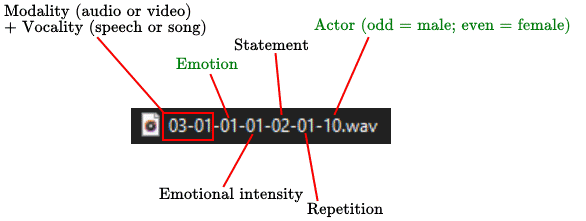
\includegraphics{figure_2_dataset_audio_example}
Figure 2 - only the sections marked in green (emotion and gender) need to be considered.
\\


\noindent Since the dataset comes labelled and is well structured, the only administrative task was to extract the key labels from each of the audio files; this was achieved through the\code{get\_label\_RAVDESS} helper function (code in the Appendix). At first glance, the emotional intensity label may seem like a factor to consider, however, due to the limitations in terms of the size of the dataset, creating additional categories would only serve to make the classification more ambiguous.
\\
\newpage

\section{Project Management}
\noindent \textbf{Gantt Chart}
\\
\noindent In order to illustrate the schedule of the project, I have produced a Gantt chart, shown below.
\\
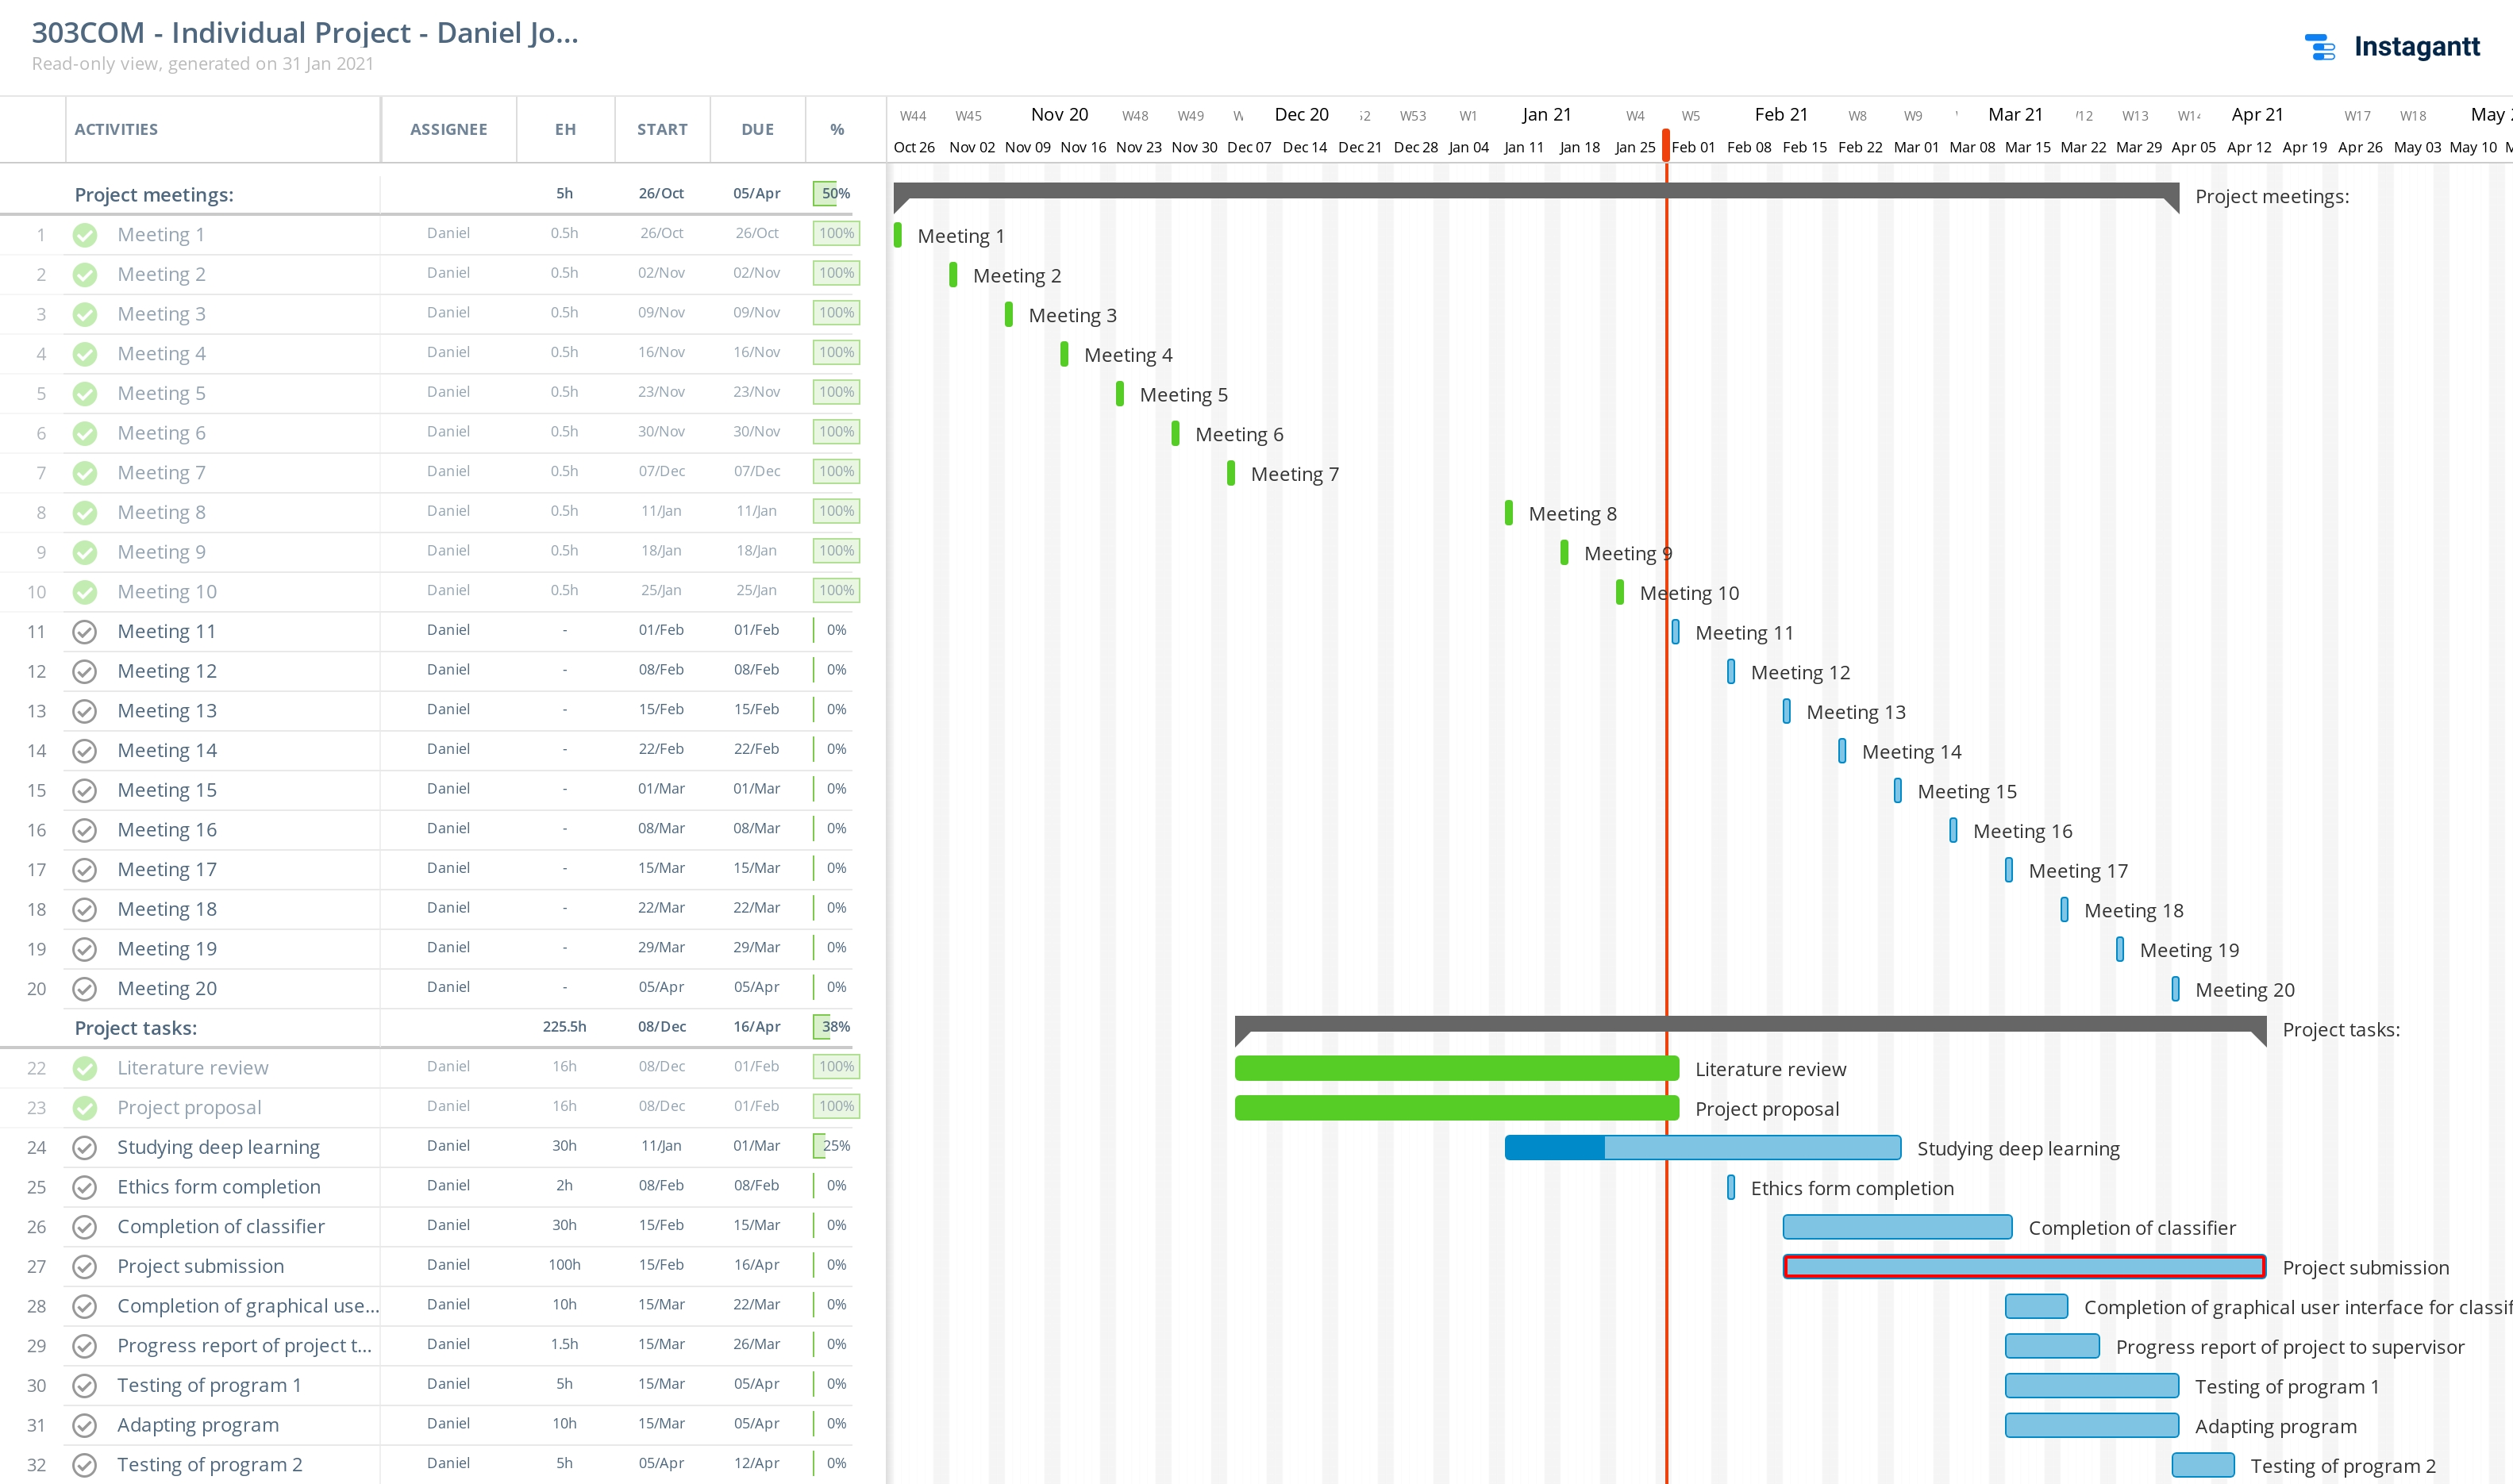
\includegraphics[width=18cm, height=12cm]{Daniel_Jones_Gantt_Chart}
\\
\noindent \href{https://i.imgur.com/9tchO4N.jpg}{\color{blue}\textbf{Link to full size image}}
\\
\noindent \href{https://app.instagantt.com/shared/s/PdaKZZeApqszVu1eftjC/latest}{\color{blue}\textbf{Link to latest edition of the chart}}
\\
\newpage

\section{References}

\begin{itemize}
\item Cho, V., Mansfield, K. C., Claughton, J. (2020). The past and future technology in classroom management and school discipline: A systematic review. \textit{Teaching and Teacher Education, 90}, 103037. \href{https://doi.org/10.1016/j.tate.2020.103037}{https://doi.org/10.1016/j.tate.2020.103037}

\item Sainath, T. N., Mohamed, A. R., Kingsbury, B., Ramabhadran, B. (2013). Deep convolutional neural networks for LVCSR. In \textit{2013 IEEE international conference on acoustics, speech and signal processing} (pp. 8614-8618). \tab \href{https://ieeexplore.ieee.org/abstract/document/6639347}{https://ieeexplore.ieee.org/abstract/document/6639347}

\item Venkataramanan, K., Rajomohan, H. R. (2019). Emotion Recognition from Speech \textit{arXiv preprint arXiv:1912.10458}. \href{https://arxiv.org/pdf/1912.10458.pdf}{https://arxiv.org/pdf/1912.10458.pdf}

\item Kerkeni, L., Serrestou, Y., Mbarki, M., Raoof, K., Mahjoub, M.A., Cleder, C. (2019). Automatic Speech Emotion Recognition Using Machine Learning. In \textit{Social media and machine learning}. IntechOpen. \href{https://doi.org/10.5772/intechopen.84856}{https://doi.org/10.5772/intechopen.84856}

\item Kwon, S. (2020). A CNN-assisted enhanced audio signal processing for speech emotion recognition. \textit{Sensors 20(1), 183}. \href{http://doi.org/10.3390/s20010183}{http://doi.org/10.3390/s20010183}

\item Harrell, S., Bynum, Y. (2018). Factors affecting technology integration in the classroom. \textit{Alabama Journal of Educational Leadership}, 5, 12-18

\item Munshi, A., Rajendran, R., Ocumpaugh, J., Biswas, G., Baker, R. S., Paquette, L. (2018). Modeling learners' cognitive and affective states to scaffold SRL in open-ended learning environments. In \textit{Proceedings of the 26th conference on user modeling, adaptation and personalization} (pp. 131-138). \tab \href{https://doi.org/10.1145/3209219.3209241}{https://doi.org/10.1145/3209219.3209241}
\end{itemize}

\newpage

\end{document}